\subsection{Modèle mathématique}\label{sec:modelMath}

Notre objectif est de déterminer le nombre moyen de machines infectées lors d'une attaque, en fonction de la configuration logicielle du système. En effet, on peut considérer que dans un système à grande échelle, avec un certain degré de redondance, une attaque n'est concluante que si un certain pourcentage des machines a été infecté. Il peut donc être plus intéressant d'optimiser le nombre moyen de machines infectées par attaque plutôt que la probabilité d'infection (c'est à dire préférer une probabilité d'infection plus importante, mais avec un faible nombre de machines infectées à chaque attaque plutôt qu'une probabilité d'infection plus faible, mais où une très grande partie du système serait affecté en cas d'attaque).\\
Pour cela, nous allons définir "l'entropie" du système. Cette grandeur vient à l'origine de la thermodynamique et caractérise le "désordre" d'un système. Claude Shannon a eu l'idée de transposer cette grandeur au domaine de la théorie de l'information\cite{entropie_shannon}.\\
Dans notre cas, nous allons reprendre sa formulation, et allons définir l'entropie de notre système comme son degré d'hétérogénéité, c'est à dire la variété des logiciels qui y sont installés pour une application donnée.
Pour cela, définissons $E_v$ comme l'ensemble des logiciels installés sur notre système de $n$ machines pour l'application fixée (e.g. un serveur web). Pour chaque élément de l'ensemble, posons $p_i$ la probabilité que ce logiciel se retrouve installé sur l'une des machines. 
On a donc:

\[
\sum_{E}p_i=1
\]

On pose alors H l'entropie de Shannon :

\[
H=-\sum_E p_i \log(p_i)
\]

On pose également $T$ comme l'ancienneté moyenne des logiciels de notre système, chaque logiciel ayant une ancienneté $T_i$ (on définit l'ancienneté d'un logiciel comme le temps écoulé depuis sa publication)  :

\[
T=\sum_E p_i T_i
\]

On recherche alors le nombre moyen d'infections par attaque en fonction de l'entropie et de l'ancienneté moyenne de notre système. En effet, on fait ici l'hypothèse simplificatrice qu'un \textit{malware} ne peut cibler qu'un unique  logiciel. Ainsi, plus notre système sera hétérogène, moins le \textit{malware} pourra se propager. En revanche, plus les versions des logiciel sont anciennes, plus le nombre de failles qui y auront été découvertes sera importante, et donc plus la probabilité d'infection initiale sera importante. Il est donc important de prendre en compte ces deux paramètres de notre système pour calculer l'importance d'une infection potentielle que l'on pose : 

\[
N_{infection} = f(H,T) = P_{attaque}(T)*D(H)
\]

En ce qui concerne la probabilité de l'infection initiale, nous considérerons par la suite qu'elle croit exponentiellement avec l'ancienneté moyenne de notre système. Nous la définissons donc comme suit :

\[
P_{attaque}(T) =1- \exp^{-\lambda*T}
\]

Si $T=0$, le logiciel vient de sortir. On considère que toutes les failles connues y ont été corrigées, et que de nouvelles failles \textit{zero day} n'y ont pas encore été découvertes. La probabilité d'infection est donc nulle. Au contraire, plus $T$ augmente, plus le nombre de failles découvertes et leur diffusion augmentent, et la probabilité d'infection tend vers 1. $\lambda$ est un paramètre qui sert à ajuster la vitesse à laquelle la probabilité d'infection augmente avec l'ancienneté du logiciel.\\

On définit $H_{un}$ comme l'entropie pour une distribution uniforme avec n logiciels différentes (chaque ordinateur a un logiciel différent) :

\[
H_{un} = -\sum_n \frac{1}{n} * \log(\frac{1}{n}) = \sum_n \frac{\log(n)}{n} = \log(n)
\]

Il reste à établir la formule reliant l'entropie et la diffusion de l'infection. Dans un premier temps, nous allons établir le mode le plus simple possible : un modèle linéaire en H. En cas d'infection, on considère que k machines sont touchées en moyenne, sur un total de m. On a alors :

\[
k=1+(m-1)*(1-\frac{H}{H_{un}}) =m-\frac{m-1}{\log(n)}*H
\]

Ce premier modèle est cohérent en $H=0$, puisqu'on est alors en présence d'un système avec un unique logiciel. En cas d'infection, $k=n$ : toutes les machines sont touchées puisqu'il n'y a pas de diversité logicielle (le \textit{malware} peut se propager partout).\\
Il est aussi cohérent pour $H=H_{un}$. En effet, chaque machine a alors un logiciel différent, et alors $k=1$ : seulement la première machine est infectée, le \textit{malware} n'arrive pas du tout à se propager.\\
La formule finale est donc :


\[
N_{infection}=[1-\exp^{-\lambda_1*T}] * [m-\frac{m-1}{\log(n)}*H]
\]

On peut remarquer que d'après notre modèle, la meilleure façon de ne pas se faire affecter est d'installer la même dernière version du logiciel sur toutes les machines, ou encore afin de ne pas propager l'infection dans le système, d'installer des logiciels différents sur chaque machine. Cela parait assez intuitif, et on peut se dire au premier abord qu'il suffit donc de se placer dans l'une ou l'autre de ces situations. Cependant, il ne faut pas oublier qu'en pratique, il est presque impossible dans un système de taille importante et en production de maintenir en permanence les logiciels à jour. De plus cela implique des coûts importants. De même, une trop grande diversité des logiciels implique un coût de maintenance élevé, puisqu'il faut préparer des procédures de mise à jour différentes pour chacun d'entre eux.
Ainsi, afin de rendre notre modèle plus réaliste, nous allons y introduire ces coûts. Il ne suffira plus alors de minimiser le taux de pénétration du \textit{malware} dans notre système, mais plutôt ce taux \textbf{plus} le coût correspondant à la maintenance du système.

Nous posons donc $C_T$ le coût de maintenance par unité de temps selon l'ancienneté moyenne des logiciels que l'on vise à avoir :

\[
C_T=m*\frac{1}{T}
\]

Ce coût est linéaire en $\frac{1}{T}$, puisque si nous voulons avoir une ancienneté moyenne des logiciels deux fois plus petite, il faudra logiquement effectuer les mises à jour deux fois plus régulièrement.

Nous posons également $C_H$ le coût de maintenance par unité de temps qui sera lui fonction de l'entropie de notre système et du nombre de logiciels qui y sont installées :

\[
C_H = g(n,H)
\]

$C_H$ dépend du nombre de logiciels dans notre système, comme expliqué précédemment, mais il dépend également de l'entropie, car si il y a uniquement une machine équipée d'une version donnée d'un logiciel, alors il suffira d'y faire une mise à jour manuelle, alors que si cette version est plus répandue, il faudra alors préparer une procédure de mise à jour automatique. Cependant,cette fonction de coût est très difficile à définir, et dépendra fortement des procédures en place dans chaque département IT. C'est pourquoi nous ne donnons pas sa forme.

Nous pouvons alors poser le coût total pour le défenseur:

\[
C_{Total}=k_1*N_{infection}+k_2*C_T+k_3*C_H
\]

Les coefficients $k_1$, $k_2$ et $k_3$ sont à définir par l'administrateur du système afin que les résultats collent à ses exigences spécifiques en terme de diffusion du \textit{malware} par rapport à ses propres coûts de maintenance informatique.

\begin{figure}[ht]
\centering
     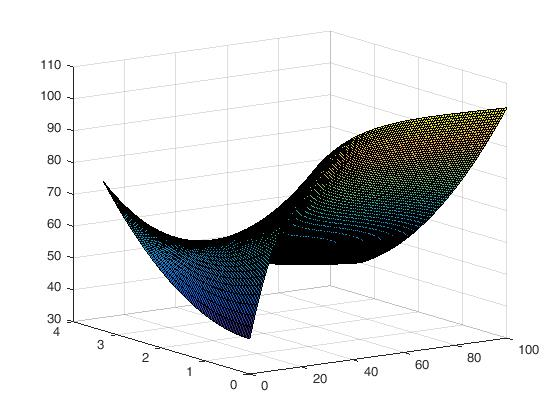
\includegraphics[width=1.0\linewidth]{Paul/Matlab/3D.jpg}
     \caption{Modélisation avec Matlab}
     \label{normal_case}
\end{figure}

\begin{figure}[ht]
\centering
     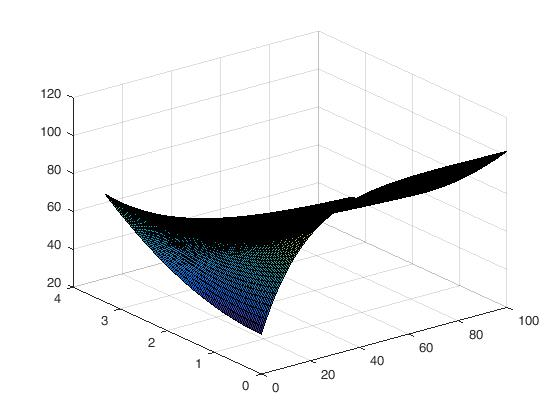
\includegraphics[width=1.0\linewidth]{Paul/Matlab/3D_proj.jpg}
     \caption{Projection de la modélisation avec Matlab}
     \label{normal_case}
\end{figure}

\begin{figure}[ht]
\centering
     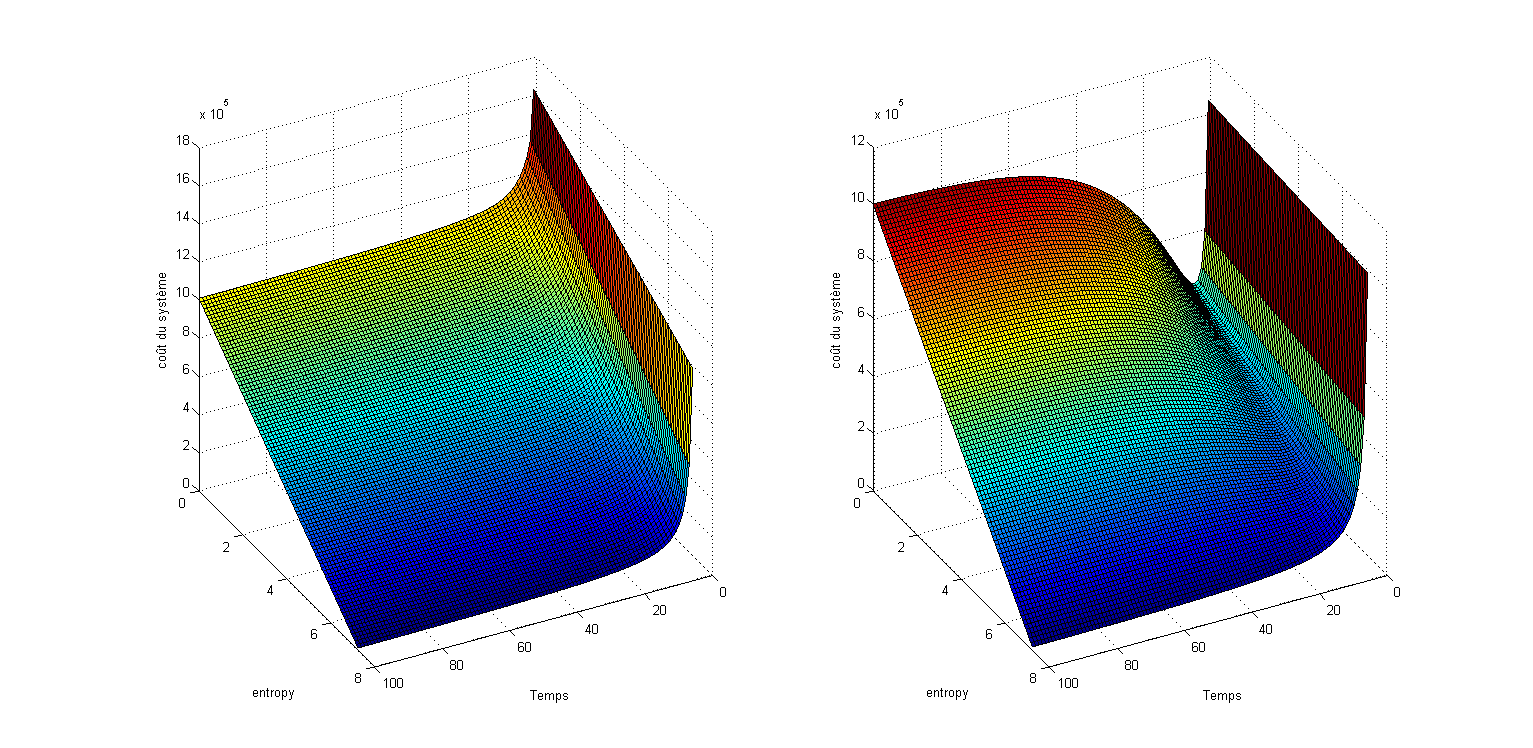
\includegraphics[width=1.0\linewidth]{Paul/Matlab/lambda_var.png}
     \caption{Impact de la variation de lambda (gauche=1, droite=0.05)}
     \label{normal_case}
\end{figure}

%Thomas : Tu peux faire la discussion des figures ici